
\section{ABB Validation and Kinematic Verification}

A series of experimental trials were conducted to verify the positional accuracy of the ABB robotic arm's nominal kinematic model. The objective was to determine if the factory-calibrated parameters were sufficient for the project's precision requirements without the need for further software-based calibration.

The experimental data collection involved measuring the end-effector's actual Cartesian coordinates against the commanded positions within the primary workspace. The resulting error statistics are detailed in Table~\ref{tab:verification_stats}.

\begin{table}[h!]
\centering
\caption{Positioning Error Statistics for Nominal Model Verification}
\label{tab:verification_stats}
\begin{tabular}{lr}
\toprule
\textbf{Error Metric} & \textbf{Value (mm)} \\ 
\midrule
Mean Error in X ($\mu_x$)           & 0.2700 \\
Mean Error in Y ($\mu_y$)           & -0.2333 \\
Mean Error Magnitude ($\|E\|$)      & 0.5052 \\
Maximum Error Magnitude ($E_{max}$) & 1.1180 \\
Standard Deviation in X ($\sigma_x$) & 0.2472 \\
Standard Deviation in Y ($\sigma_y$) & 0.4028 \\ 
\bottomrule
\end{tabular}
\end{table}



As the data illustrates, the Mean Error Magnitude ($0.5052$~mm) is remarkably low for a standard industrial manipulator in an uncalibrated state. These results fall strictly within the manufacturer’s specified tolerance for this model. Because the residual errors were found to be negligible for the intended manipulation tasks, it was concluded that the nominal kinematic parameters are highly reliable. Consequently, further kinematic calibration was deemed unnecessary, and the system was validated for immediate use in high-level control applications.

\begin{figure}[H]
    \vspace{-15pt}
    \centering
    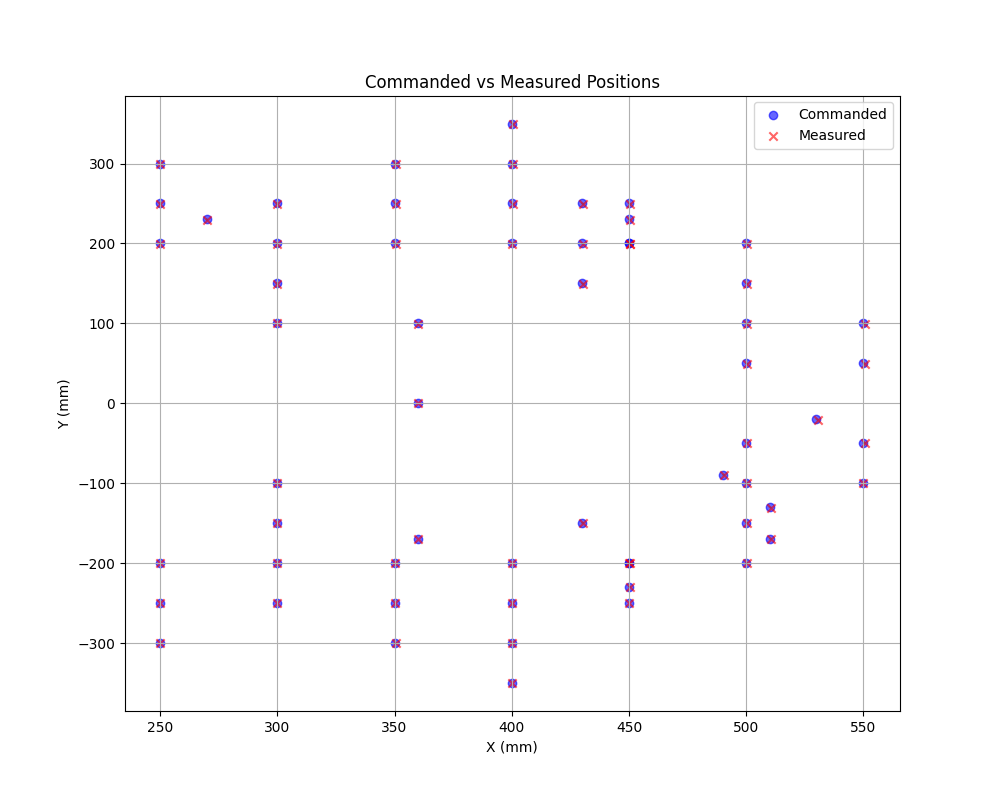
\includegraphics[width=0.7\textwidth]{Figures/chapter3/ABB validation/validation_abb.png} 
    \vspace{-15pt}
    \caption{Distribution of measured positional errors confirming factory accuracy.}
    \label{fig:validation_plot}
\end{figure}
